\documentclass[11pt]{article}
\usepackage[margin=1in]{geometry}
\usepackage{volfit_preamble}
\graphicspath{{figures/}}

\title{\textbf{Bayesian Prior Persistence}\\[2pt]
\large Trust the market where it speaks, the prior where it does not\\[2pt]
\normalsize Vol-Fitter Technical Notes, No.~13}
\author{Vol-Fitter}
\date{\today}

\begin{document}
\maketitle
% Auto-generated by gen_prior.py — do not edit.
\newcommand{\priatmmarket}{39.9}
\newcommand{\priatmprior}{31.5}
\newcommand{\priatmpersist}{40.7}
\newcommand{\priwingprior}{41.7}
\newcommand{\priwingmo}{52.6}
\newcommand{\priwingps}{40.6}
\newcommand{\priunmet}{59}


\begin{abstract}
A desk does not re-derive its volatility surface from scratch each morning: it
\emph{persists} yesterday's surface and lets today's quotes update it. Done
naively this is a dilemma. Load the prior too hard and you \emph{damp} a real
overnight signal --- an ATM vol that genuinely jumped gets pulled back toward
yesterday. Load it too softly and the sparsely-quoted wings \emph{flap}, over-fit
to a steep ATM skew. This note documents the Vol-Fitter's resolution: a Bayesian
prior-persistence framework built on one idea --- an \emph{activation gate} that
turns the prior \emph{off} exactly where today's quotes already identify a feature,
and \emph{on} where they do not. We give the universal residual form and the gate
$\mathrm{gap}=\max(1-\text{obs}/\text{req},0)^\gamma$, the shared precision
vocabulary (quote density, bid--ask width, freshness, transport distance), and the
seven persistence modes --- off, overlay, strike gaps, quote operators, smile
factors, hybrid (the default), and graph-only --- including why the
risk-reversal/butterfly operators must be \emph{signed baskets} to preserve their
coupling. A worked example, built with the production calibrator, shows an ATM jump
of $+8$ vol points preserved (the persisted ATM is \priatmpersist\%, tracking the
market, not the calmer prior's \priatmprior\%) while an unquoted wing is held at the
prior ($\priwingps\%$ vs the market-only fit's wild $\priwingmo\%$). An empirical
temporal backtest confirms the hybrid default reconstructs held-out wings
$\sim32$ vol bps better than no prior, two-thirds of the time.
\end{abstract}

\tableofcontents
\newpage

%======================================================================
\section{The morning dilemma}
\label{sec:dilemma}

Overnight, two things change unevenly. The at-the-money level may move sharply on
fresh news, and it is \emph{well quoted} --- the liquid near-the-money options
re-price immediately. The wings, by contrast, may have \emph{no} fresh quotes at
all, yet they still need values. A fitter faces a choice:

\begin{itemize}[leftmargin=1.4em]
\item \textbf{Re-fit from today's quotes only.} The ATM is captured, but with no
wing quotes the model extrapolates the (now steeper) ATM skew into the wings,
producing implausible tails --- the wings \emph{flap}.
\item \textbf{Anchor hard to yesterday's prior.} The wings are stabilized, but the
prior also pulls the \emph{ATM} back toward yesterday, \emph{damping} the real
overnight signal.
\end{itemize}

\begin{heuristic}
The resolution is to make the prior's strength \emph{local} and
\emph{data-aware}: strong in the wings (no quotes $\Rightarrow$ trust yesterday),
zero at the money (fresh quotes $\Rightarrow$ trust today). The same prior, applied
through a gate that reads how well today's data identifies each feature, gives both
behaviours at once. This is just Bayesian updating with a precision that depends on
the observation density --- but stated as an operational rule: \emph{do not damp the
signal.}
\end{heuristic}

%======================================================================
\section{The universal residual and the activation gate}
\label{sec:gate}

Every persistence mode adds residuals of one shape: a difference between a
\emph{functional} of the model and the same functional of the prior, scaled by a
data-aware weight,
\begin{equation}
\boxed{\;r_j=\sqrt{\lambda_j}\,\frac{O_j(\text{model})-O_j(\text{prior})}{\text{scale}_j},
\qquad
\lambda_j=\underbrace{\text{strength}}_{\text{global}}\cdot\underbrace{\pi^{\text{prior}}_j}_{\text{prior precision}}\cdot\underbrace{\mathrm{gap}_j}_{\text{gate}}.\;}
\label{eq:universal}
\end{equation}
$O_j$ is a strike price, an operator (ATM/RR/BF), or a local smile factor depending
on the mode (\cref{sec:modes}). The decisive factor is the \emph{activation gate}
\begin{equation}
\mathrm{gap}_j=\max\!\Big(1-\frac{\pi^{\text{obs}}_j}{\pi^{\text{req}}_j},\,0\Big)^{\!\gamma},
\label{eq:gap}
\end{equation}
where $\pi^{\text{obs}}_j$ is how precisely today's quotes identify coordinate $j$
and $\pi^{\text{req}}_j$ the precision at which the prior should switch off. When
the data meets or exceeds the requirement, $\mathrm{gap}_j=0$ and the prior
contributes \emph{nothing}; when the data says nothing, $\mathrm{gap}_j\to1$ and
the prior is at full strength. The exponent $\gamma$ sharpens the transition.
\Cref{fig:gate} plots it.

\begin{figure}[H]
\centering
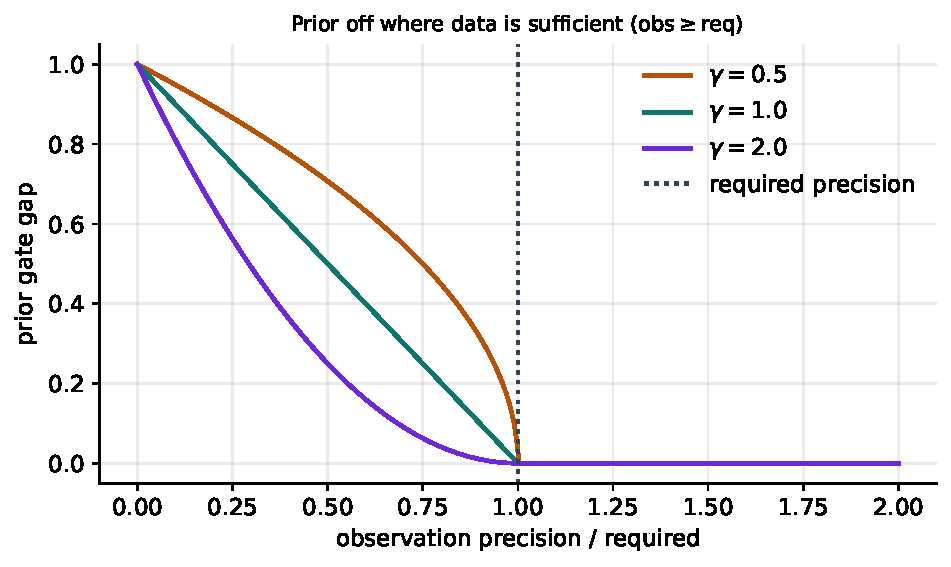
\includegraphics[width=0.72\textwidth]{fig_prior_gate.pdf}
\caption{The activation gate \eqref{eq:gap}. Past the required precision the prior
weight is exactly zero --- the ``do not damp the signal'' rule. $\gamma$ controls
how hard the on/off edge is.}
\label{fig:gate}
\end{figure}

%======================================================================
\section{The precision vocabulary}
\label{sec:precision}

The gate needs a shared notion of precision, used identically by every mode (and
by the graph baseline of Note~14). A raw precision is scaled by model-agnostic
factors in $(0,1]$:
\begin{itemize}[leftmargin=1.4em]
\item \textbf{Fit quality} $1/\text{rms}^2$, floored at a $1$-vol-bp excellence
level (a great fit is precise, not infinitely so).
\item \textbf{Quote density} --- more supporting quotes raise precision, saturating
at a reference count ($\sim8$ near-ATM quotes for full credit).
\item \textbf{Bid--ask width} --- precision halves at a relative spread of $\sim5\%$
of ATM vol.
\item \textbf{Freshness} --- exponential decay with quote/prior age (half-lives of a
few days for observations, $\sim30$ days for the prior).
\item \textbf{Transport distance} --- a prior transported a forward distance
$|h|=|\log(F_{\text{now}}/F_{\text{prior}})|$ is less trustworthy, decaying on a
scale of $\sim10\%$.
\end{itemize}
The \emph{observation} precision (data side) combines fit quality, density,
spread and freshness; the \emph{prior} precision (baseline side) combines
provenance, age and transport. Both carry per-handle floors and caps so that one
excellent fit cannot dominate and one stale prior cannot vanish entirely.

%======================================================================
\section{The seven modes}
\label{sec:modes}

The mode (\texttt{priorPersistenceMode}) chooses the functional $O_j$ in
\eqref{eq:universal}.

\begin{enumerate}[leftmargin=1.6em]
\item \textbf{Off.} No prior penalty and no overlay --- a pure current-market fit.
\item \textbf{Overlay.} The transported prior is \emph{drawn} (dotted) for
reference but exerts no calibration pull.
\item \textbf{Strike gaps.} $O_j$ is the call price at a spread of delta-locations.
The weight follows the \emph{data-gap} density: $\rho_{\text{desired}}(x)-\rho_{\text{observed}}(x)$,
the positive part, where $\rho_{\text{observed}}$ is a Gaussian kernel density of
the live quotes and $\rho_{\text{desired}}$ is the coverage we want spread over the
\emph{wider} delta span. A region already sampled to the desired density gets zero
prior weight; only the deficit (sparse wings, gaps) is filled. This is the mode in
the worked example.
\item \textbf{Quote operators.} $O_j\in\{\text{ATM},\text{RR}_{25},\text{BF}_{25},\text{VarSwap}\}$,
persisted only where today's quotes do not identify the operator. RR and BF must be
\emph{signed baskets} (\cref{sec:baskets}).
\item \textbf{Smile factors.} $O_j\in\{\text{ATM},\text{skew},\text{curvature},\dots\}$,
ATM-local finite-difference stencils --- the prior's \emph{shape} re-expressed at
the current node.
\item \textbf{Hybrid (default).} Operator priors (ATM/RR/BF/var-swap) plus a
residual deep-tail strike anchor only where no operator covers --- the empirically
best reconstruction (\cref{sec:validation}).
\item \textbf{Graph-only.} The prior enters \emph{only} as the graph baseline for
extrapolation (Note~14); dark nodes receive propagated innovations rather than a
direct anchor.
\end{enumerate}

\subsection{Why operators are signed baskets}
\label{sec:baskets}

A risk-reversal or butterfly is a \emph{combination} of leg vols, not a single
quote. Persisting RR and BF as \emph{per-leg} prices would silently drop their
coupling --- the prior would anchor the legs independently and lose ``the skew
should persist'' as a joint statement. Instead each operator is a signed linear
functional (basket) of the leg implied vols (parametric) or of the leg call prices
(local-vol), giving \emph{one} residual per operator that preserves the RR/BF
coupling on whatever surface the model draws. This also fixed a long-standing
asymmetry: the SVI and Multi-Core SIV overlays, which previously received no prior
at all, now get the same signed-operator treatment as LQD.

%======================================================================
\section{Two-pass activation}
\label{sec:twopass}

The gate \eqref{eq:gap} needs the observation precision, which in its sharpest form
is the \emph{realized} fit quality --- a chicken-and-egg with the fit it modifies.
The optional two-pass mode (\texttt{priorDataOnlyPrepass}) resolves it cleanly:
fit once on data alone, measure each operator's realized precision, then refit with
priors active only on the under-observed coordinates. This is the most faithful
``do not damp'' behaviour but costs $\sim2\times$ per node, so it is opt-in; the
default single pass gates by quote-support precision with no extra fit.

%======================================================================
\section{Worked example: an overnight jump}
\label{sec:example}

\Cref{fig:nodamp} is the dilemma made concrete, built with the production strike-gap
prior and calibrator. Yesterday's prior is a calm $\priatmprior\%$-ATM smile.
Overnight the market jumps: today's ATM is $\priatmmarket\%$ with a steeper skew,
and \emph{only} the ATM region ($|k|\le0.10$) is quoted. The market-only fit
captures the ATM but extrapolates the steep skew into a wild put wing
($\priwingmo\%$ at $k=-0.30$). The prior-persisted fit keeps the ATM essentially
at the \emph{market} level (\priatmpersist\%, tracking the market's
\priatmmarket\% rather than being damped toward the prior's \priatmprior\%) because the gate is zero where the quotes are dense, while holding
the unquoted wing at the prior ($\priwingps\%$, vs the prior's $\priwingprior\%$)
because the gate is one where there are no quotes. The signal is preserved; the gap
is filled.

\begin{figure}[H]
\centering
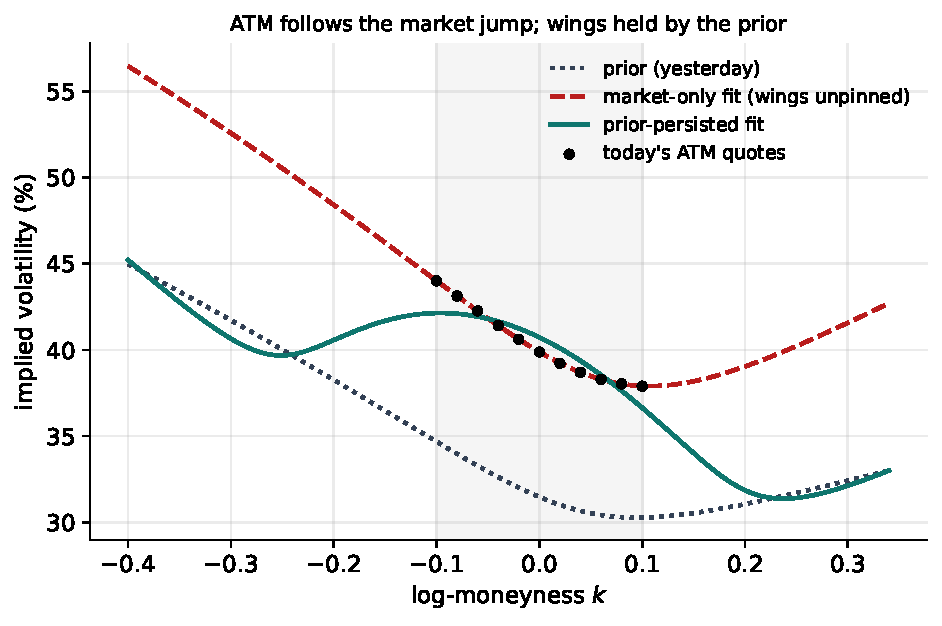
\includegraphics[width=0.82\textwidth]{fig_prior_nodamp.pdf}
\caption{``Don't damp the signal.'' The persisted fit (solid) tracks the market ATM
jump (quoted region shaded) while the unquoted wings are held by the prior (dotted),
rather than flapping like the market-only fit (dashed).}
\label{fig:nodamp}
\end{figure}

%======================================================================
\section{Empirical validation}
\label{sec:validation}

The framework is validated by a \emph{temporal} backtest. For each
$(\text{asset},\,T{-}1\to T)$ pair it fits day $T{-}1$'s full chain, freezes it as
the active prior, thins day $T$ to its ATM region, refits under each mode, and
scores the reconstructed \emph{held-out} moderate wing against the true day-$T$
quotes (with \texttt{off} as the baseline). Over the full spike regime ($1117$
nodes plus a bandwidth/probe sweep), the shipped \textbf{hybrid} default
reconstructs the held-out wing $\sim32$ vol bps better than no prior, $\sim66\%$ of
the time, and wins at \emph{every} bandwidth and var-swap probe tested; the
strike-gap mode is a close second, while the pure signed-operator modes do not beat
\texttt{off} at the median --- the reconstruction comes from the tail/strike anchor,
not the signed RR/BF operators. The backtest thus \emph{confirmed} the shipped
configuration rather than changing a default: the operator bandwidth is not a
productive lever (left at $0.06$) and the var-swap probe stays at $1.4\sigma$.

%======================================================================
\section{What is original here}
\label{sec:original}

The Bayesian framing (prior precision $\times$ data precision) is standard; the
contributions are the \emph{operational} pieces. The \emph{activation gate}
\eqref{eq:gap} turns ``do not damp the signal'' into one differentiable factor
shared by every mode. The \emph{shared precision vocabulary} means strike gaps,
operators, factors and the graph baseline all speak the same language of
confidence. The \emph{signed-basket} operators \eqref{sec:baskets} keep the RR/BF
coupling that per-leg persistence would lose, and incidentally cured the
overlay-models' missing-prior asymmetry. And the \emph{two-pass} option closes the
fit-quality circularity exactly. The whole framework is byte-identical to a plain
fit when the mode is \texttt{off}, so persistence is strictly additive.

\appendix
%======================================================================
\section{Hyperparameter atlas}
\label{app:atlas}

\begin{longtable}{p{0.30\textwidth}p{0.14\textwidth}p{0.48\textwidth}}
\caption{Prior-persistence hyperparameters.}\label{tab:atlas}\\
\toprule Knob & Default & Role\\ \midrule
\endfirsthead \toprule Knob & Default & Role\\ \midrule \endhead
\multicolumn{3}{l}{\emph{Surfaced (OptionsSettings)}}\\ \midrule
\texttt{priorPersistenceMode} & \texttt{hybrid} & The mode selector (\cref{sec:modes}).\\
\texttt{priorAnchorWeightPct} & $50\%$ & Strike-gap budget (fraction of option weight).\\
\texttt{priorAnchorDeltas} & $\{2,5,10,25,40\}\Delta$ & Delta-locations for strike anchors.\\
\texttt{priorOperatorSet} & ATM/RR25/BF25/VS & Operators to persist.\\
\texttt{priorOperatorStrengthPct} & $50\%$ & Operator budget.\\
\texttt{priorOperatorRequiredPrecision} & $1.0$ & Gate threshold $\pi^{\text{req}}$.\\
\texttt{priorOperatorGapExponent} $\gamma$ & $1.0$ & Gate sharpness.\\
\texttt{priorOperatorBandwidth} & $0.06$ & Operator leg KDE bandwidth.\\
\texttt{priorFactorSet} & ATM/skew/curv/VS & Smile factors to persist.\\
\texttt{priorFactorStrengthPct} & $50\%$ & Factor budget.\\
\texttt{priorTailAnchorStrengthPct} & $20\%$ & Hybrid deep-tail anchor budget.\\
\texttt{priorDataOnlyPrepass} & off & Two-pass activation (\cref{sec:twopass}).\\
\midrule
\multicolumn{3}{l}{\emph{Hidden (precision vocabulary)}}\\ \midrule
\texttt{RMS\_FLOOR} & $10^{-4}$ & Fit-quality precision floor (1 vol bp).\\
\texttt{REF\_ATM\_QUOTES} & $8$ & Quote count for full density credit.\\
\texttt{SPREAD\_HALF} & $0.05$ & Relative spread at which precision halves.\\
\texttt{OBS/PRIOR\_FRESHNESS\_HALFLIFE} & $3$\,/\,$30$\,d & Freshness/age half-lives.\\
\texttt{TRANSPORT\_SCALE} & $0.10$ & Transport-distance precision scale.\\
\texttt{DEFAULT\_BANDWIDTH} & $0.06$ & Observed-quote KDE bandwidth.\\
\texttt{MAX\_INV\_VEGA\_RATIO} & $25$ & Cap on deep-wing vega amplification.\\
\texttt{\_VARSWAP\_PROBE\_STD} & $1.4\sigma$ & Var-swap coverage probe half-width.\\
\bottomrule
\end{longtable}

\noindent\textbf{Performance.} The prior blocks add a few residual rows and bump
the options version (one refit on change). The single-pass gate is free (it reuses
quote-support density); the two-pass prepass costs $\sim2\times$ per node and is
opt-in. Mode \texttt{off} is byte-identical to a plain fit.

\begin{thebibliography}{9}
\bibitem{Gelman2013} A.~Gelman et al. \emph{Bayesian Data Analysis}. CRC Press,
3rd ed., 2013.
\bibitem{Gatheral2006} J.~Gatheral. \emph{The Volatility Surface}. Wiley, 2006.
\bibitem{Tikhonov1977} A.~Tikhonov and V.~Arsenin. \emph{Solutions of Ill-Posed
Problems}. Winston, 1977.
\end{thebibliography}

\end{document}
